%!TEX TS-program = xelatex
\documentclass{EdipyLabs} % Custom class provided for EDIPY labs.
\SetLabNumber{8}
\SetLabTitle{Εικονικά Τοπικά Δίκτυα (VLAN)}
\SetAuthor{Χρήστος Δαλαμάγκας}
\SetLabDescription{Εικονικά Τοπικά Δίκτυα (VLAN), συγκαναλώσεις (trunk), 802.1Q, δρομολόγηση inter-vlan, router-on-a-stick, Dynamic Trunking Protocol (DTP), VLAN Trunk Protocol (VTP).}
\SetLabPrerequisites{Εργαστηριακά φυλλάδια 2α, 2β και 3 (Διευθέτηδη δρομοογητή, Διευθέτηση μεταγωγέα, Υποδικτύωση IPv4).}

\begin{document}
\Initialize

\section*{Εισαγωγή}
Αντικείμενο του παρόντος εργαστηριακού φυλλαδίου αποτελεί η μελέτη των VLAN και του πρωτοκόλλου 802.1Q, καθώς και των πρωτοκόλλων VTP και DTP. H εργαστηριακή άσκηση αποτελείται από δυο σενάριο, στο πρώτο θα εφαρμόσετε βασικές ρυθμίσεις παραμετροποίησης VLAN και στο δεύτερο σενάριο θα επικεντρωθείτε στα πρωτόκολλα VTP και DTP. Η γενική άποψη της τοπολογίας που θα υλοποιήσετε στο πλαίσιο της εργαστηριακής άσκησης φαίνεται στο σχήμα \ref{fig:generic}.

\begin{figure}[ht]
	\centering
	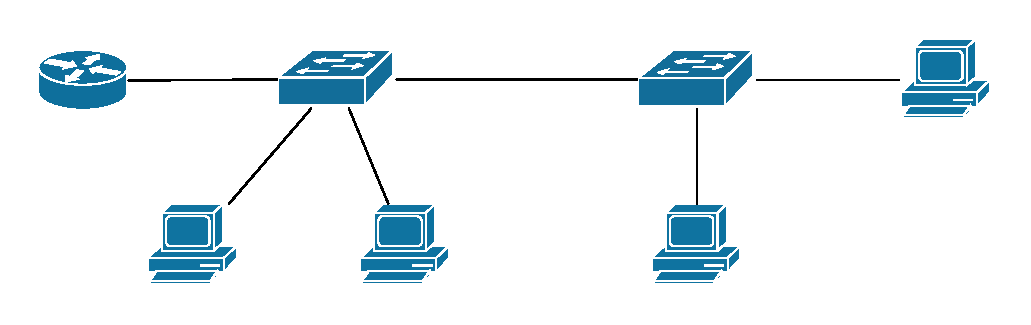
\includegraphics[width=0.75\linewidth]{generic-topology}
	\caption{Η γενική άποψη της τοπολογίας προς υλοποίηση.}\label{fig:generic}
\end{figure}

Για την υλοποίηση της τοπολογίας θα χρειαστείτε τις εξής συσκευές:
\begin{itemize}
	\item x2 Cisco Catalyst 2960.
	\item x1 Cisco 2921.
	\item x4 υπολογιστές.
\end{itemize}

\section{Θεωρητικό υπόβαθρο}

Ο τομέας ευρυεκπομπής (broadcast domain) καθορίζεται από όλες εκείνες τις δικτυακές συσκευές μιας τοπολογίας που λαμβάνουν ένα πλαίσιο, όταν αυτό ευρυεκπέμπεται. Αναφερόμενοι σε δρομολογητές, κάθε διεπαφή ανήκει σε διαφορετικό τομέα ευρυεκπομπής, σε αντίθεση με τους μεταγωγείς, οι θύρες των οποίων είναι γεφυρωμένες (bridged), δηλαδή ανήκουν στον ίδιο τομέα ευρυεκπομπής.

Σε μεγαλύτερα δικτυακά περιβάλλοντα με εκατοντάδες σταθμούς εργασίας, οι οποίοι συνδέονται σε ένα πλήθος μεταγωγέων, υπάρχει η ανάγκη τεμαχισμού του φυσικού τομέα ευρυεκπομπής και οργάνωσης των σταθμών εργασίας σε πολλαπλούς λογικούς τομείς ευρυεκπομπής. O λογικός διαχωρισμός ενός τομέα επιτυγχάνεται με τα Εικονικά Τοπικά Δίκτυα (Virtual Local Area Networks - VLANs). Στο σχήμα \ref{fig:grouping} απεικονίζεται ένα παράδειγμα διαχωρισμού του φυσικού τομέα ευρυεκπομής σε τρία VLAN. 

\begin{figure}[ht]
	\centering
	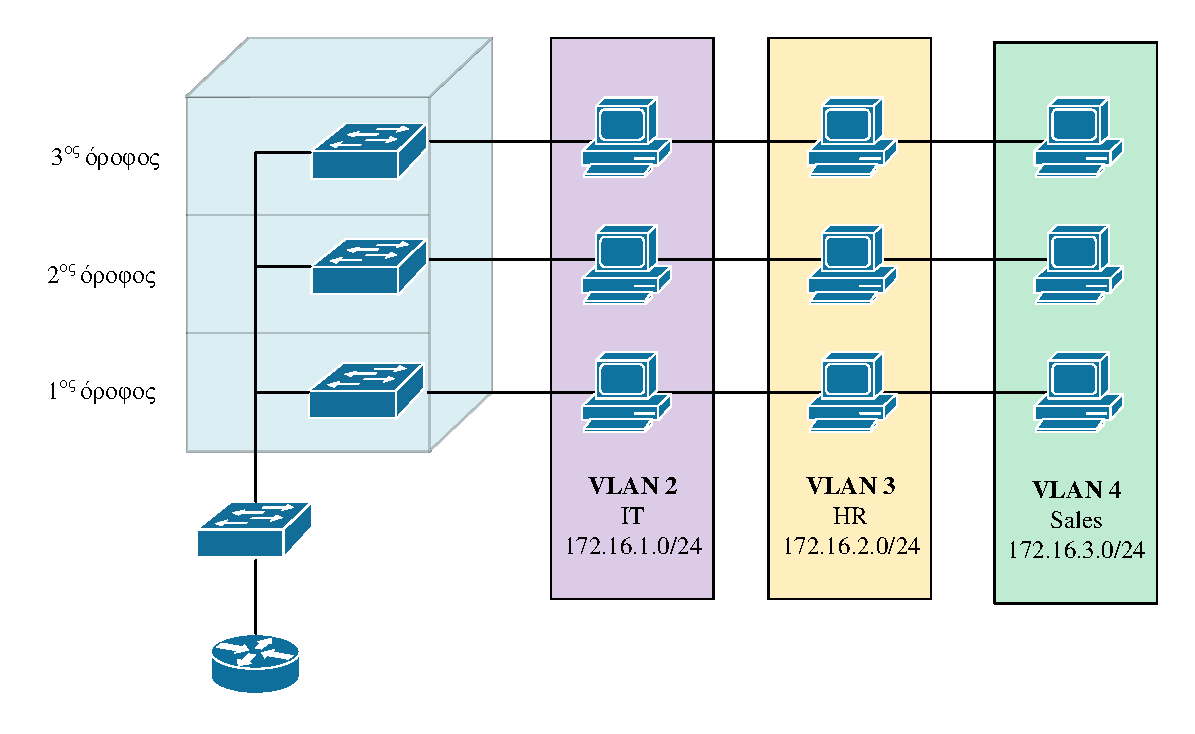
\includegraphics[width=0.75\linewidth]{vlan-example}
	\caption{Παράδειγμα ομαδοποίησης υπολογιστών σε VLAN.}\label{fig:grouping}
\end{figure}

Όπως φαίνεται και στο σχήμα \ref{fig:grouping}, κάθε VLAN αποτελεί ένα απομονωμένο δίκτυο, τόσο στο δεύτερο στρώμα του OSI όσο και στο τρίτο, κάτι το οποίο είναι εμφανές από τη διαφορετική διευθυνσιοδότηση που έχει κάθε VLAN. Τα VLAN επιτρέπουν την ομαδοποίηση των υπολογιστών, ακόμη και αν αυτοί βρίσκονται σε διαφορετικούς φυσικούς χώρους και συνδέονται απευθείας με διαφορετικούς μεταγωγείς. Στο σχήμα φαίνεται ότι τα τρία VLAN που έχουν οριστεί διαθέτουν μέλη και στους τρεις ορόφους του κτηρίου.  

Σε κάθε θύρα ενός μεταγωγέα που βρίσκεται σε \textbf{κατάσταση πρόσβασης} (access mode) μπορεί να ανατεθεί αποκλειστικά ένα VLAN. Για παράδειγμα, στο σχήμα \ref{fig:grouping}, η θύρα του μεταγωγέα του τρίτου ορόφου, στην οποία συνδέεται ο υπολογιστής του VLAN 2, έχει ρυθμιστεί κατάλληλα ώστε να εξυπηρετεί πλαίσια αποκλειστικά για το VLAN 2. Τυχόν μήνυμα ευρυεκπομπής που προέλθει από κάποιον υπολογιστή του VLAN 2, θα μεταδοθεί μόνο από τις θύρες του μεταγωγέα που εξυπηρετούν το VLAN 2. 

Οι ζεύξεις μεταξύ των μεταγωγέων δύναται να μεταφέρουν πλαίσια που ανήκουν σε διαφορετικά VLAN. Σε αυτή την περίπτωση, οι αντίστοιχες θύρες τίθενται σε \textbf{κατάσταση συγκανάλωσης} (trunking mode), με τις αντίστοιχες ζεύξεις να αποκαλούνται «\textit{συγκαναλώσεις}» (trunks). 

\subsection{To πρωτόκολλο 802.1Q}
O λογικός διαχωρισμός ενός φυσικού τομέα ευρυεκπομπής σε VLAN υλοποιείται με τη χρήση ετικετών VLAN (VLAN tagging), οι οποίες τοποθετούνται ως πεδία στα πλαίσια ethernet. Το πιο ευρέως χρησιμοποιούμενο πρωτόκολλο για τις ετικέτες VLAN είναι το 802.1q της IEEE. Στο σχήμα απεικονίζεται η μορφή ενός πλαισίου ethernet με την ετικέτα 802.1q.

\begin{figure}[ht]
	\centering
	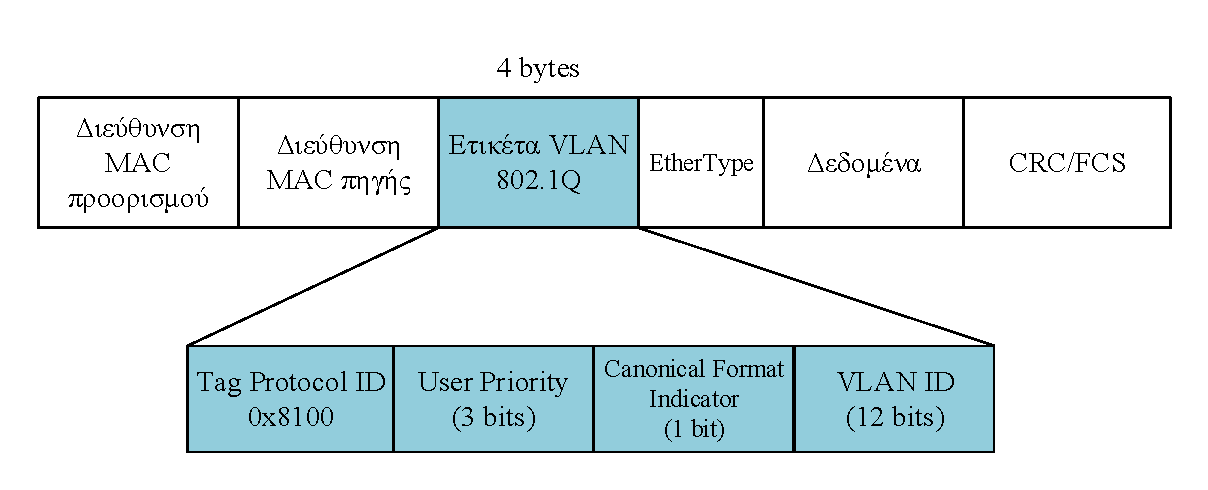
\includegraphics[width=0.75\linewidth]{dot8021q}
	\caption{Η ετικέτα ΙΕΕΕ 802.1q σε ένα πλαίσιο ethernet.}\label{fig:dot8021q}
\end{figure}

Μια ετικέτα VLAN 802.1q αποτελείται από τα εξής πεδία:
\begin{itemize}
	\item \textbf{Tag Protocol ID} (TPID): Αφορά το πρωτόκολλο στρώματος σύνδεσης δεδομένων, στο οποίο έχει προστεθεί η ετικέτα. Για το Ethernet η τιμή του πεδίου είναι 0x8100.
	\item \textbf{User priority}: Το πεδίο χρησιμοποιείται για την υποστήριξη ποιότητας υπηρεσιών.
	\item \textbf{Canonical Format Identifier (CFI)}: Το πεδίο επιτρέπει την μετάδοση πλαισίων Token Ring σε δίκτυα ethernet.
	\item \textbf{VLAN ID}: Ένας αριθμός 12 bit που αντιπροσωπεύει την ταυτότητα ενός VLAN.
\end{itemize}

Με βάση το αναγνωριστικό τους, τα VLAN διακρίνονται στις εξής κατηγορίες:
\begin{itemize}
	\item \textbf{Προεπιλεγμένο VLAN} (default VLAN): Όλες οι θύρες ενός μεταγωγέα ανατίθενται από εργοστασιακές ρυθμίσεις στο προεπιλεγμένο VLAN. To προεπιλεγμένο VLAN για τους μεταγωγείς Cisco είναι το VLAN 1. Οι βέλτιστες πρακτικές ασφαλείας συστήνουν την ανάθεση των ανενεργών θυρών, που δεν χρησιμοποιούνται από κάποια συσκευή, σε ένα οποιοδήποτε VLAN που δεν χρησιμοποιείται. Το VLAN αυτό αποκαλείται «μαύρη τρύπα» (blackhole VLAN).
	\item \textbf{Εγγενές VLAN} (native VLAN): To εγγενές VLAN χρησιμοποιείται για λόγους συμβατότητας με μεταγωγείς που δεν υποστηρίζουν ετικέτες VLAN και ανατίθεται σε όσα πλαίσια προέρχονται από αυτούς τους μεταγωγείς, τη στιγμή που διέρχονται από μια συγκανάλωση. Από προεπιλογή, το εγγενές ταυτίζεται με το προεπιλεγμένο VLAN. Οι βέλτιστες πρακτικές ασφαλείας συνιστούν την αλλαγή του εγγενούς VLAN με κάποιο που δεν χρησιμοποιείται ήδη.\footnote{H αλλαγή του εγγενούς VLAN βοηθάει στην αντιμετώπιση της επίθεσης διπλής ετικέτας (double tagging).}
	\item \textbf{VLAN δεδομένων} (data VLAN): Ονομάζεται έτσι οποιοδήποτε VLAN έχει ανατεθεί σε μια ή περισσότερες θύρες ενός μεταγωγέα και χρησιμοποιείται για τη μετάδοση δεδομένων που παράγουν οι χρήστες.
	\item \textbf{Διαχειριστικό VLAN} (management VLAN): Ονομάζεται έτσι οποιοδήποτε VLAN, στην SVI του οποίου έχει ανατεθεί διεύθυνση IP και μάσκα υποδικτύου. Από προεπιλογή, το διαχειριστικό VLAN είναι το VLAN 1. Οι βέλτιστες πρακτικές ασφαλείας συνιστούν την αλλαγή του διαχειριστικού VLAN με κάποιο που δεν χρησιμοποιείται ήδη.
\end{itemize}

Ακόμη, με βάση το αναγνωριστικό τους, η Cisco διαχωρίζει τα VLAN σε δυο πρόσθετες κατηγορίες:
\begin{itemize}
	\item \textbf{VLAN κανονικού εύρους} (normal range VLANs): Είναι όσα έχουν αναγνωριστικό από 1 μέχρι 1005. Οι παραμετροποιήσεις που αφορούν τα κανονικά VLAN αποθηκεύονται στο αρχείο \textbf{vlan.dat} που βρίσκεται στη μνήμη flash.
	\item \textbf{VLAN εκτεταμένου εύρους} (extended range VLANs): Είναι όσα έχουν αναγνωριστικό από 1006 μέχρι 4094. Υποστηρίζουν λιγότερα χαρακτηριστικά σε σύγκριση με τα κανονικά VLAN και οι παραμετροποιήσεις που αφορούν τα εκτεταμένα VLAN αποθηκεύονται στις τρέχουσες ρυθμίσεις. 
\end{itemize}

\subsection{Βασική παραμετροποίηση VLAN}

Η δημιουργία ενός VLAN σε έναν μεταγωγέα γίνεται από την κατάσταση ρυθμίσεων με τις εντολές που παρατίθενται στον πίνακα \ref{tab:commands-vlan-create}.

\begin{CommandTable*}{Εντολές για τη δημιουργία ενός VLAN.}{commands-vlan-create}{7cm}{9cm}
	S1\#\textbf{configure terminal} & Είσοδος σε καθολική κατάσταση ρύθμισης.\\
	S1(config)\#\textbf{vlan} \textit{vlan-id}  & Δημιουργία ενός VLAN με τον προσδιορισμό ενός αναγνωριστικό.\\
	S1(config-vlan)\#\textbf{name} \textit{vlan-name} & Προσδιορισμός ενός μοναδικού ονόματος για την αναγνώριση του VLAN.\\
	S1(config-vlan)\#\textbf{end} & Επιστροφή στην κατάσταση επαυξημένων δικαιωμάτων.
\end{CommandTable*}

Αν και οι ρυθμίσεις για τα κανονικά VLAN αποθηκεύονται στο αρχείο vlan.dat της μνήμης flash, ωστόσο αν υπάρχει η επιθυμία να διατηρηθούν οι ρυθμίσεις των VLAN μόνιμα, προτείνεται η αποθήκευση των τρεχουσών ρυθμίσεων με την εντολή \ip{copy run start}. 

Επόμενο βήμα της δημιουργίας ενός VLAN είναι η ανάθεση θυρών σε αυτό, η οποία γίνεται από την κατάσταση ρύθμισης διεπαφής, με τις εντολές που παρατίθενται στον πίνακα \ref{tab:commands-vlan-assign}.

\begin{CommandTable}{Εντολές για την ανάθεση VLAN σε θύρες μεταγωγέα.}{commands-vlan-assign}
	S1\#\textbf{configure terminal} & Είσοδος σε καθολική κατάσταση ρύθμισης.\\
	S1(config)\#\textbf{interface} \textit{interface\_id} & Επιλογή της διεπαφής προς ρύθμιση. Η εντολή \ip{interface range} θα μπορούσε να χρησιμοποιηθεί για ταυτόχρονη επιλογή περισσότερων θυρών.\\
	S1(config-if)\#\textbf{switchport mode access} & Ορισμός της διεπαφής σε κατάσταση πρόσβασης. Η εντολή είναι προαιρετική, ωστόσο συνίσταται η χρήση της για λόγους ασφαλείας.\\
	S1(config-if)\#\textbf{switchport access vlan} \textit{vlanid} & Ανάθεση της επιλεγμένης θύρας σε ένα VLAN.\\
	S1(config-if)\#\textbf{end} & Επιστροφή στην κατάσταση επαυξημένων δικαιωμάτων.
\end{CommandTable}

Με την εντολή \ip{show vlan brief} μπορείτε να προβάλλετε τα VLAN που έχουν δημιουργηθεί σε έναν μεταγωγέα, καθώς και τις θύρες που έχουν ανατεθεί σε κάθε ένα από αυτά. Στο παράδειγμα που ακολουθεί φαίνεται πως σε όλες τις θύρες πλην της Fa0/10 έχει ανατεθεί το VLAN 1. Στο VLAN 10 με όνομα student έχει ανατεθεί η θύρα Fa0/5.

\begin{CommandBox}
`Switch\#\textbf{show vlan brief}
\begin{longtable}{lllp{5cm}}
	VLAN &Name                             &Status    &Ports\\
	---- &-------------------------------- &--------- &-------------------\\
	1    &default                          &active    &Fa0/1, Fa0/2, Fa0/3, Fa0/4, Fa0/6, Fa0/7, Fa0/8, ...\\
	\hl{10}   &\hl{student}                &\hl{active}    &\hl{Fa0/5}\\
	1002 &fddi-default                     &active    &\\
	1003 &token-ring-default               &active    &\\
	1004 &fddinet-default                  &active    &\\
	1005 &trnet-default                    &active    &
\end{longtable}`
\end{CommandBox}

H διαγραφή ενός συγκεκριμένου VLAN γίνεται με την εντολή: \ip{S1(config)\#\textbf{no vlan} \textit{vlan-id}}.

\warningbox{Πριν διαγράψετε ένα VLAN, πρώτα αναθέστε τις θύρες του σε κάποιο άλλο ήδη υπαρκτό VLAN. Σε διαφορετική περίπτωση ενδέχεται να εμφανιστούν προβλήματα συνδεσιμότητας στους χρήστες.}

Σε αντίθεση με τις θύρες σε κατάσταση πρόσβασης, οι θύρες σε κατάσταση συγκανάλωσης επιτρέπουν την μεταφορά πλαισίων από πολλά VLAN. Ο ορισμός μιας θύρας σε κατάσταση συγκανάλωσης επιτυγχάνεται με τις εντολές του πίνακα \ref{tab:commands-trunk}. Πληροφορίες για τις συγκαναλώσεις ενός μεταγωγέα μπορείτε να λάβετε με την εντολή \ip{show interfaces trunk}.

\begin{CommandTable}{Εντολές για την παραμετροποίηση συγκαναλώσεων σε μεταγωγέα.}{commands-trunk}
	S1\#\textbf{configure terminal} & Είσοδος σε καθολική κατάσταση ρύθμισης.\\
	S1(config)\#\textbf{interface} \textit{interface\_id} & Επιλογή της διεπαφής προς ρύθμιση.\\
	S1(config-if)\#\textbf{switchport mode trunk} & Ορισμός της διεπαφής σε κατάσταση συγκανάλωσης.\\
	S1(config-if)\#\textbf{switchport trunk native vlan} \textit{vlan-id} &  \textit{Προαιρετικό}. Αλλαγή του εγγενούς VLAN.\\
	S1(config-if)\#\textbf{switchport trunk allowed vlan} \textit{vlan-list} & Ορισμός των VLAN που επιτρέπεται να χρησιμοποιήσουν τη θύρα συγκανάλωσης\footnotemark.\\
	S1(config-if)\#\textbf{end} & Επιστροφή στην κατάσταση επαυξημένων δικαιωμάτων.
\end{CommandTable}

Επισημαίνεται ότι όταν μια θύρα ορίζεται σε κατάσταση συγκανάλωσης, τότε επιτρέπεται η διέλευση πλαισίων από οποιοδήποτε VLAN. Αυτή η προεπιλεγμένη λειτουργία των συγκαναλώσεων εγκυμονεί κινδύνους ασφαλείας, αυτό προτείνεται ο ρητός προσδιορισμός των επιτρεπόμενων VLAN σε μια συγκανάλωση με την εντολή \texttt{\textbf{switchport trunk allowed vlan} \textit{vlan-list}}.

Δεδομένου ότι τα VLAN ανήκουν σε διαφορετικούς τομείς ευρυεκπομπής, χρειάζεται ένας δρομολογητής ή μεταγωγέας στρώματος 3 (layer 3 switch), που να δρομολογεί τα πακέτα μεταξύ των VLAN. Η ρύθμιση router-on-the-stick είναι η πιο δημοφιλής επιλογή για δρομολόγηση μεταξύ VLAN (inter-vlan routing), κατά την οποία δημιουργούνται υποδιεπαφές (subinterfaces) σε μια φυσική διεπαφή του δρομολογητή, με κάθε υποδιεπαφή να αντιστοιχίζεται σε διαφορετικό VLAN. 

Στο παράδειγμα που ακολουθεί δημιουργούνται δυο υποδιεπαφές στη διεπαφή GigabitEthernet 0/0, στις οποίες ανατίθενται τα VLAN 5 και 10. Η τεχνική του router-on-a-stick συνοψίζεται στα εξής βήματα:\label{inter-vlan}
\begin{itemize}
	\item Αρχικά, δημιουργείται η υποδιεπαφή με την εντολή \ip{interface} \texttt{\textit{interface\_id}.\textit{subinterface\_id}}. Ως αριθμό της υποδιεπαφής μπορεί να οριστεί οποιοσδήποτε αριθμός, ωστόσο συνήθης πρακτική είναι το αναγνωριστικό της υποδιεπαφής να ταυτίζεται με το VLAN ID που η υποδιεπαφή εξυπηρετεί. 
	\item Με την εντολή \ip{encapsulation dot1q} \texttt{\textit{vlan-id}} ορίζεται το είδος της ενθυλάκωσης στρώματος 2 που πρέπει να χρησιμοποιήσει η υποδιεπαφή (802.1Q για την περίπτωση των VLAN), μαζί με το VLAN ID που εξυπηρετεί η υποδιεπαφή. 
	\item Εφαρμόζεται η επιθυμητή διευθυνσιοδότηση IP με την εντολή \ip{ip address}. 
	\item Όταν δημιουργηθούν όλες οι υποδιεπαφές, ενεργοποιείται η φυσική διεπαφή με την εντολή \ip{no shutdown}. 
\end{itemize}

\begin{CommandBox}
R1(config)#`\textbf{interface g0/0.5}`
R1(config-subif)#`\textbf{encapsulation dot1q 5}`
R1(config-subif)#`\textbf{ip address 192.168.5.1 255.255.255.0}`
R1(config-subif)#`\textbf{interface g0/0.10}`
R1(config-subif)#`\textbf{encapsulation dot1q 10}`
R1(config-subif)#`\textbf{ip address 192.168.10.1 255.255.255.0}`
R1(config-subif)#`\textbf{interface g0/0}`
R1(config-if)#`\textbf{no shutdown}`
\end{CommandBox}

\footnotetext{Τα επιτρεπόμενα VLAN ID στην εντολή παρατίθενται διαχωρισμένα με κόμμα. Για παράδειγμα, η εντολή \texttt{switchport trunk allowed vlan 10,20,30} επιτρέπει τη διέλευση των VLAN 10, 20 και 30 από τη συγκανάλωση.}
\newpage

\subsection{To πρωτόκολλο VTP}
Όσο μεγαλώνει ο αριθμός των μεταγωγέων σε ένα δίκτυο, η δημιουργία, διαγραφή και διαχείριση των υπαρχόντων VLAN αποτελεί μια δύσκολη διαδικασία. Η Cisco απλοποίησε τη διαδικασία αυτή με το VLAN Trunking Protocol (VTP). Το πρωτόκολλο απλοποιεί τη διαχείριση των VLAN, με τη διάδοση των υπαρχόντων VLAN των εξυπηρετητών VTP προς τους υπόλοιπους μεταγωγείς μιας τοπολογίας. Συνοπτικά, το πρωτόκολλο αποτελείται από τα εξής συστατικά:
\begin{itemize}
	\item \textbf{Τομέας VTP} (VTP domain): Αποτελείται από έναν ή περισσότερους διασυνδεδεμένους μεταγωγείς και οριοθετείται από έναν δρομολογητή ή μεταγωγέα επιπέδου 3. Οι μεταγωγείς που ανήκουν στον ίδιο τομέα μοιράζονται πληροφορίες σχετικά με τα VLAN που γνωρίζουν χρησιμοποιώντας διαφημίσεις VTP.
	\item \textbf{Διαφημίσεις VTP} (VTP advertisments): Κάθε μεταγωγέας στέλνει περιοδικά τις πληροφορίες για τα VLAN που γνωρίζει μέσω των συγκαναλώσεών του προς τη διεύθυνση πολυδιανομής 01-00-0C-CC-CC-CC. Οι μεταγωγείς από τον ίδιο τομέα που λαμβάνουν τις διαφημίσεις ενημερώνουν τις δικές τους ρυθμίσεις VLAN. Οι διαφημίσεις VTP χαρακτηρίζονται από τον τομέα VTP και τον αριθμό αναθεώρησης (revision number). Όταν γίνεται οποιαδήποτε αλλαγή σχετική με VLAN σε έναν εξυπηρετητή VTP, τότε παράγεται διαφήμιση με αριθμό αναθεώρησης αυξημένο κατά 1. Μεγαλύτερη τιμή του αριθμού αναθεώρησης υποδηλώνει πιο πρόσφατη ενημέρωση, καθώς και την υποχρέωση του μεταγωγέα που την λαμβάνει να αναθεωρήσει κατάλληλα τις ρυθμίσεις VLAN.
	\item \textbf{Κωδικός VTP} (VTP Password): Κατά τη δημιουργία ενός νέου τομέα VTP, μπορεί να οριστεί κωδικός πρόσβασης, τον οποίο πρέπει να εισαγάγουν οι μεταγωγείς που θέλουν να εισέλθουν στον ίδιο τομέα.
	\item \textbf{Καταστάσεις VTP} (VTP Modes): Ένας μεταγωγέας δύναται να λειτουργήσει στις εξής καταστάσεις VTP:
	\begin{itemize}
		\item \textbf{Εξυπηρετητής VTP} (VTP Server): Διαφημίζει τις πληροφορίες VLAN που διαθέτει προς όλους τους μεταγωγείς του ίδιου τομέα VTP. Μπορεί να δημιουργεί, να διαγράφει και να τροποποιεί τα VLAN του τομέα στον οποίον ανήκει. Οι ρυθμίσεις σχετικά με τα VLAN αποθηκεύονται στο αρχείο \texttt{vlan.dat} της NVRAM. Κάθε μεταγωγέας λειτουργεί από προεπιλογή σε κατάσταση εξυπηρετητή, στον τομέα NULL. 
		\item \textbf{Πελάτης VTP} (VTP Client): Διαφημίζει τις πληροφορίες VLAN που διαθέτει προς όλους τους μεταγωγείς του ίδιου τομέα VTP. Δεν μπορεί να δημιουργήσει, να διαγράψει ή να τροποποιήσει τα VLAN που μαθαίνει από τις διαφημίσεις. Οι ρυθμίσεις σχετικά με τα VLAN αποθηκεύονται στις τρέχουσες ρυθμίσεις της RAM. 
		\item \textbf{Διαφανές VTP} (VTP transparent): Οι μεταγωγείς αυτής της κατηγορίες απλώς προωθούν τις διαφημίσεις που λαμβάνουν προς τις συγκαναλώσεις τους. Τροποποιήσεις που αφορούν τα VLAN παραμένουν στη συσκευή και δεν διαφημίζονται προς τους υπόλοιπους μεταγωγείς.
	\end{itemize}
\end{itemize}
Εναλλακτικό ανοικτό πρότυπο του VTP αποτελεί το Multiple VLAN Registration Protocol (MVRP), το οποίο όμως δεν είναι διαθέσιμο στις δικτυακές συσκευές του εργαστηρίου. 

\subsection{To πρωτόκολλο DTP}

Το ιδιόκτητο πρωτόκολλο DTP (Dynamic Trunking Protocol) χρησιμοποιείται αποκλειστικά από τους μεταγωγείς της Cisco για την αυτόματη διαπραγμάτευση της κατάστασης λειτουργίας των θυρών. Ανάλογα με την κατάσταση που βρίσκεται μια θύρα του μεταγωγέα Α και την κατάσταση της έτερης θύρας στον μεταγωγέα Β, αποφασίζεται από το πρωτόκολλο DTP η τελική κατάσταση μιας θύρας. Στον πίνακα απεικονίζεται το αποτέλεσμα της διαπραγμάτευσης ανάλογα με την κατάσταση που βρίσκονται οι θύρες. Ακολουθεί μια σύντομη περιγραφή της κάθε κατάστασης με την παράθεση της αντίστοιχης εντολής που ενεργοποιεί την εν λόγω λειτουργία:
\begin{itemize}
	\item \ip{switchport mode access}: Ορίζει τη διεπαφή σε μόνιμη κατάσταση πρόσβασης και προσπαθεί πολύ ενεργά να μετατρέψει την απέναντι θύρα στην ίδια κατάσταση.
	\item \ip{switchport mode dynamic auto}: Θέτει τη θύρα σε μια «παθητική» κατάσταση, κατά την οποία η θύρα μπορεί να δεχτεί μετατροπή σε συγκανάλωση, αν η απέναντι θύρα το επιθυμεί. Η θύρα έχει μια ελαφρά επιθυμία να μετατρέψει τη ζεύξη σε κατάσταση πρόσβασης. Αυτή είναι η προεπιλεγμένη κατάσταση για κάθε θύρα των μεταγωγέων της Cisco. 
	\item \ip{switchport mode dynamic desirable}: Κάνει την θύρα να προσπαθεί ενεργά να μετατρέψει τη ζεύξη σε συγκανάλωση, χωρίς ωστόσο να αποκλείεται το γεγονός να μετατραπεί σε κατάστση πρόσβασης, αν η απέναντι θύρα είναι σε μόνιμη κατάσταση πρόσβασης.
	\item \ip{switchport mode trunk}: Ορίζει τη διεπαφή σε μόνιμη κατάσταση συγκανάλωσης και προσπαθεί πολύ ενεργά να μετατρέψει την απέναντι θύρα στην ίδια κατάσταση.
\end{itemize}

Λόγω του γεγονότος πως το DTP δεν παρέχει μηχανισμούς ασφαλείας, ένας κακόβουλος χρήστης μπορεί να διεξάγει την επίθεση switch spoofing, δηλαδή να στείλει κατασκευασμένα πλαίσια DTP, προσποιούμενος ότι είναι μεταγωγέας, με σκοπό να αποκτήσει πρόσβαση στα VLAN που επιτρέπονται από τη συγκανάλωση. Για την αντιμετώπιση της εν λόγω επίθεσης συνίσταται ο χειροκίνητος καθορισμός της κατάστασης λειτουργίας (συγκανάλωση ή πρόσβαση) και η απενεργοποίηση του πρωτοκόλλου DTP με την εντολή \ip{switchport nonegotiate}.

\begin{table}[ht]
	\centering\renewcommand{\arraystretch}{1.25}
	\begin{adjustbox}{width=\textwidth, center}
	\begin{tabular}{lllll}
		\FormatFirstRow
			 						& \textbf{Dynamic Auto} & \textbf{Dynamic Desirable} & \textbf{Trunk} & \textbf{Access}	\\
		\textbf{Dynamic Auto}		& Access				& Trunk						 & Trunk		  & Access			\\
		\textbf{Dynamic Desirable}	& Trunk					& Trunk						 & Trunk		  & Access			\\
		\textbf{Trunk}				& Trunk					& Trunk						 & Trunk		  & Περ/μένη συνδ/τητα\\
		\textbf{Access}				& Access				& Access					 & Περ/μένη συνδ/τητα & Access
	\end{tabular}
	\end{adjustbox}
\caption{Τα αποτελέσματα των διαπραγματεύσεων του DTP}\label{tab:dtp}
\end{table}

\section{Προετοιμασία δικτύου}\label{sec:2}

\begin{figure}[H]
	\centering
	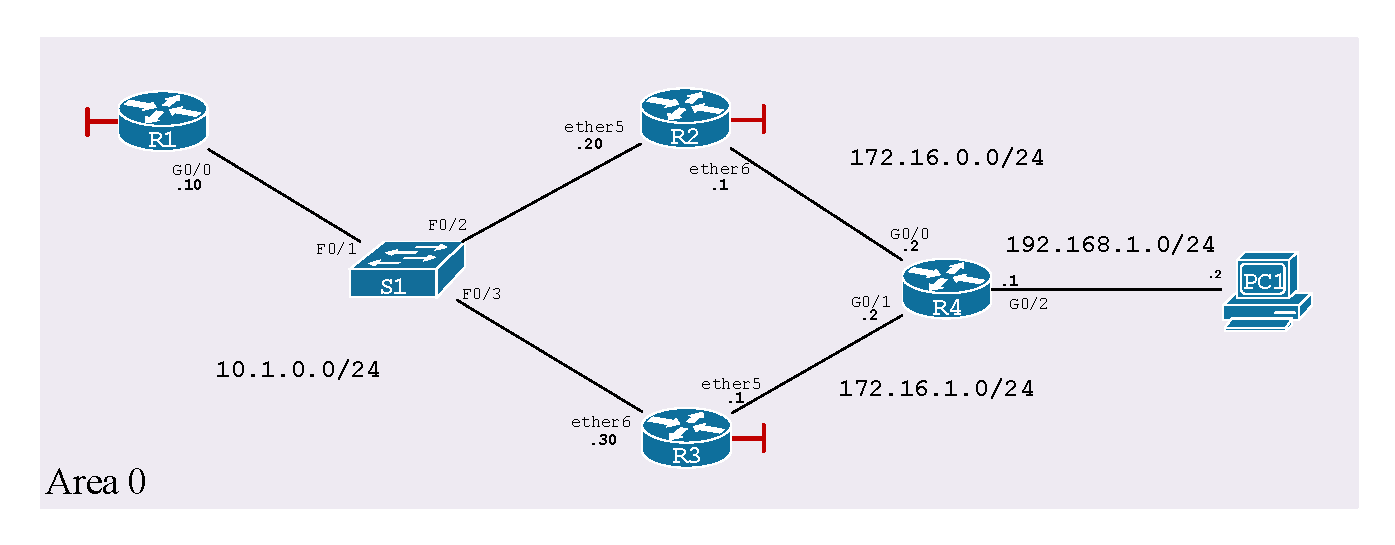
\includegraphics[width=\linewidth]{topology-1}
	\caption{Το σχέδιο της αναλυτικής τοπολογίας προς υλοποίηση.}\label{fig:topology-1}
\end{figure}

\begin{IpAddressTable}{Το σχήμα διευθυνσιοδότησης της τοπολογίας.}{iptable-1}
	& \ip{Gi0/0.10}	& \ip{192.168.10.1}		& \ip{255.255.255.0}	& \\
	& \ip{Gi0/0.20} & \ip{192.168.20.1}		& \ip{255.255.255.0}    & \\
	& \ip{Gi0/0.88} & \ip{192.168.88.1}		& \ip{255.255.255.0}    & \\
	\multirow{-4}{*}{R1}& \ip{Gi0/0.99} & \ip{192.168.99.1}		& \ip{255.255.255.0}	& \multirow{-3}{*}{-}\\
	\rowcolor{lightgray}
	S1	& SVI			& \ip{192.168.88.251}	&  \ip{255.255.255.0}   & \ip{192.168.88.1} \\
	S2	& SVI			& \ip{192.168.88.252}	&  \ip{255.255.255.0}   & \ip{192.168.88.1} \\
	\rowcolor{lightgray}
	PC1	& NIC			& \ip{192.168.10.5}		&  \ip{255.255.255.0}   & \ip{192.168.10.1} \\
	PC2	& NIC			& \ip{192.168.20.5}		&  \ip{255.255.255.0}   & \ip{192.168.20.1} \\				
	\rowcolor{lightgray}									    
	PC3	& NIC			& \ip{192.168.20.6}		&  \ip{255.255.255.0}   & \ip{192.168.20.1} \\				
	PC4	& NIC			& \ip{192.168.1.5}		&  \ip{255.255.255.0}   & \ip{192.168.1.1}
\end{IpAddressTable}%
\begin{VlanTable}{Το σχήμα ανάθεσης VLAN.}{vlantable-1}
	10						& Student 						& S1: \ip{Fa0/0/5} - \ip{Fa0/0/10} \\
	\rowcolor{lightgray}    
	&  								& S1: \ip{Fa0/0/15} - \ip{Fa0/0/20} \\
	\rowcolor{lightgray}						
	\multirow{-2}{*}{20}	& \multirow{-2}{*}{Faculty}		& S2: \ip{Fa0/0/15} - \ip{Fa0/0/20} \\
	&								& S1: SVI		\\
	\multirow{-2}{*}{88}    & \multirow{-2}{*}{Management}	& S2: SVI\\
	\rowcolor{lightgray}
	90						& Blackhole						& Οι θύρες που δεν χρησιμοποιούνται.\\
\end{VlanTable}

Ακολουθήστε τα εξής βήματα για την προετοιμασία του δικτύου της εργαστηριακής άσκησης:
\begin{itemize}
	\item Υλοποιήστε τη συνδεσμολογία που απεικονίζεται στο σχήμα της τοπολογίας.
	\item Βεβαιωθείτε ότι οι δικτυακές συσκευές λειτουργούν στις εργοστασιακές ρυθμίσεις. Αν βλέπετε ότι έχουν ήδη δημιουργθεί VLAN, διαγράψτε τα με την εντολή \ip{delete vlan.dat}, διαγράψτε το αρχείο ρυθμίσεων της NVRAM με την εντολή \ip{write erase} και κάνετε \ip{reload}.
	\item Αναθέστε διευθύνσεις IP στους υπολογιστές, σύμφωνα με το σχήμα διευθυνσιοδότησης.
	\item Ακολουθώντας τις βέλτιστες πρακτικές ασφαλείας, απενεργοποιήστε διαχειριστικά (\ip{shutdown}) όλες τις θύρες που δεν χρησιμοποιούνται.
\end{itemize}

\section{Σενάριο: Δρομολόγηση μεταξύ VLAN}
Στο πρώτο σενάριο θα εφαρμόσετε βασικές παραμετροποιήσεις VLAN. Συγκεκριμένα, θα δημιουργήσετε VLAN στους μεταγωγείς και θα ενεργοποιήσετε τη δρομολόγηση μεταξύ των VLAN με τη μέθοδο router on a stick.

\subsection{Δημιουργία και παραμετροποίηση των VLAN}

Ξεκινώντας, με βάση τον πίνακα \ref{tab:vlantable-1} δημιουργήστε τα VLAN 10, 20 και 88 στους μεταγωγείς της τοπολογίας. Για παράδειγμα, με τις ακόλουθες εντολές μπορείτε να δημιουργήσετε το VLAN 10 στον μεταγωγέα S1 και να το μετονομάσετε σε Student.

\begin{CommandBox}
S1#`\textbf{configure terminal}`
S1(config)#`\textbf{vlan 10}`
S1(config-vlan)#`\textbf{name Student}`
S1(config-vlan)#`\textbf{exit}`
\end{CommandBox}

\subsection{Ανάθεση των θυρών σε VLAN}

Αφού δημιουργήσετε τα VLAN, αναθέστε τις θύρες των μεταγωγέων στα VLAN σύμφωνα με τον πίνακα \ref{tab:vlantable-1}. Εκτελέστε τις ακόλουθες εντολές στον S1 για να αναθέσετε στις θύρες FastEthernet0/0/5 μέχρι FastEthernet0/0/10 το VLAN 10. Ακόμη, ακολουθώντας τις βέλτιστε πρακικές, απενεργοποιήστε την αυτόματη διαπραγμάτευση του DTP για τις θύρες αυτές με την εντολή \ip{switchport nonegotiate}: 

\begin{CommandBox}
S1#(config)`\textbf{interface range fa0/0/5 - 10}`
S1(config-if-range)#`\textbf{switchport mode access}`
S1(config-if-range)#`\textbf{switchport access vlan 10}`
S1(config-if-range)#`\textbf{switchport nonegotiate}`
S1(config-if-range)#`\textbf{exit}`
\end{CommandBox}

Δώστε τις αντίστοιχες εντολές στον S2 για την επιθυμητή παραμετροποίηση.


\subsection{Ρύθμιση των συγκαναλώσεων}
Για να διακινούνται πλαίσια 802.1Q από πολλά VLAN στην τοπολογία, όσο και πλαίσια που έρχονται χωρίς ετικέτα, θα πρέπει οι κατάλληλες θύρες να οριστούν σε κατάσταση συγκανάλωσης. Παρατηρήστε την τοπολογία και διακρίνετε εκείνες τις θύρες των μεταγωγέων που μεταφέρουν πλαίσια από πολλά VLAN. Ορίστε τις αντίστοιχες θύρες σε κατάσταση συγκανάλωσης, συμβουλευόμενοι τις εντολές του πίνακα \ref{tab:commands-trunk}.

Ακολουθώντας τις βέλτιστες πρακτικές ασφαλείας, ορίστε ως εγγενές VLAN το 99. Ακόμη, σε κάθε συγκανάλωση απενεργοποιήστε την αυτόματη διαπραγμάτευση του DTP με την εντολή \ip{switchport nonegotiate} της κατάστασης ρύθμισης διεπαφής.

\warningbox{Παρατηρήστε πως στη θύρα του PC4 δεν ορίσατε κάποιο VLAN, άρα αυτή ανήκει στο προεπιλεγμένο VLAN. Συνεπώς, στα επιτρεπόμενα VLAN των συγκαναλώσεων θα χρειαστεί να προσθέσετε και το προεπιλεγμένο VLAN.}

\subsection{Ρύθμιση των SVI}
Για τα VLAN 88 των μεταγωγέων, αναθέστε τις διευθύνσεις IP που παρατίθεται στο σχήμα διευθυνσιοδότησης. Θυμηθείτε ότι μέσω των SVI έχουν πρόσβαση οι διαχειριστές στις γραμμές VTY με χρήση των πρωτοκόλλων SSH/Telnet. Ενδεικτικά, για τον S1 μπορείτε να εκτελέσετε τις εξής εντολές:

\begin{CommandBox}
S1#(config)`\textbf{interface vlan 88}`
S1(config-vlan)#`\textbf{ip address 192.168.88.251 255.255.255.0}`
S1(config-vlan#`\textbf{no shutdown}`
S1(config-vlan)#`\textbf{ip default-gateway 192.168.88.1}`
S1#
\end{CommandBox}

\subsection{Ρύθμιση της δρομολόγησης μεταξύ των VLAN}
Χρησιμοποιήστε την τεχνική router on a stick στον δρομολογητή της τοπολογίας για να ενεργοποιήστε τη δρομολόγηση μεταξύ των VLAN. Με βάση τις οδηγίες της σελίδας \pageref{inter-vlan} δημιουργήστε τις υποδιεπαφές 1, 10, 20 και 88, εφαρμόζοντας τη διευθυνσιοδότηση του πίνακα \ref{tab:iptable-1}.

Ο πίνακας δρομολόγησης πρέπει να έχει την εξής μορφή:

\begin{CommandBox}
R1>`\textbf{show ip route}`
Gateway of last resort is not set

     192.168.1.0/24 is variably subnetted, 2 subnets, 2 masks
C       192.168.1.0/24 is directly connected, GigabitEthernet0/0.1
L       192.168.1.1/32 is directly connected, GigabitEthernet0/0.1
     192.168.10.0/24 is variably subnetted, 2 subnets, 2 masks
C        192.168.10.0/24 is directly connected, GigabitEthernet0/0.10
L       192.168.10.1/32 is directly connected, GigabitEthernet0/0.10
     192.168.20.0/24 is variably subnetted, 2 subnets, 2 masks
C       192.168.20.0/24 is directly connected, GigabitEthernet0/0.20
L       192.168.20.1/32 is directly connected, GigabitEthernet0/0.20
     192.168.88.0/24 is variably subnetted, 2 subnets, 2 masks
C       192.168.88.0/24 is directly connected, GigabitEthernet0/0.88
L       192.168.88.1/32 is directly connected, GigabitEthernet0/0.88
\end{CommandBox} 

\subsection{Δοκιμές συνδεσιμότητας}
Στείλτε πακέτα ICMP μεταξύ των υπολογιστών της τοπολογίας και επιβεβαιώστε τη σωστή παραμετροποίηση του δικτύου. Θα πρέπει να επικοινωνούν οι υπολογιστές που ανήκουν σε διαφορετικά VLAN, μέσω του δρομολογητή.
\newpage

\section{Σενάριο: Τα πρωτόκολλα VTP και DTP}
Στο δεύτερο σενάριο της εργαστηριακής άσκησης θα εστιάσετε στην αυτόματη διαχείριση των VLAN με το πρωτόκολλο VTP, καθώς και της κατάστασης συγκανάλωσης των θυρών με το πρωτόκολλο DTP. 

\subsection{Επαναφορά ρυθμίσεων}
Ξεκινώντας, επαναφέρετε τις εργοστασιακές ρυθμίσεις \textbf{μόνο} για τους μεταγωγείς, διαγράφοντας ταυτόχρονα τα VLAN που δημιουργήσατε. Για την επαναφορά δώστε τις εντολές του δεύτερου bullet της ενότητας \ref{sec:2}.

\subsection{Ορισμός εξυπηρετητή VTP}
Ο εξυπηρετητής VTP της τοπολογίας είναι ο μεταγωγέας που γνωρίζει όλα τα VLAN και τα γνωστοποιεί στους υπόλοιπους μεταγωγείς του ίδιου τομέα VTP μέσω διαφημίσεων. Με τις ακόλουθες εντολές, ορίστε ως εξυπηρετητή VTP τον S1, αλλάξτε τον τομέα VTP σε UOWM και ορίστε ως κωδικό ασφαλείας τη λέξη uowm.

\begin{CommandBox}
S1(config)#`\textbf{vtp domain UOWM}`
Changing VTP domain name from NULL to UOWM
*Au 8 00:00:00.000: %SW_VLAN-6-VTP_DOMAIN_NAME_CHG: VTP domain name 
changed to UOWM.
S1(config)#`\textbf{vtp mode server}`
Device mode already VTP Server for VLANS.
S1(config)#`\textbf{vtp password uowm}`
Setting device VTP password to uowm
\end{CommandBox}

Με την ακόλουθη εντολή επιβεβαιώστε ότι η παραμετροποίηση του εξυπηρετητή VTP αντιστοιχεί στις εντολές που εκτελέσατε.

\begin{CommandBox}
S1#`\textbf{show vtp status}`
VTP Version                     : 2
Configuration Revision          : 0
Maximum VLANs supported locally : 255
Number of existing VLANs        : 6
`\hl{VTP Operating Mode}`              : `\hl{Server}`
`\hl{VTP Domain Name}`                 : `\hl{UOWM}`
VTP Pruning Mode                : Disabled
VTP V2 Mode                     : Disabled
VTP Traps Generation            : Disabled
MD5 digest                      : 0xA1 0x1B 0x37 0x00 0x7C 0xC6 0x1B 0x94 
Configuration last modified by 0.0.0.0 at 3-1-93 00:02:29
Local updater ID is 0.0.0.0 (no valid interface found)
S1#
\end{CommandBox}

\subsection{Ορισμός πελάτη VTP}
Ο εξυπηρετητής VTP της τοπολογίας είναι ο μεταγωγέας που γνωρίζει όλα τα VLAN και τα γνωστοποιεί στους υπόλοιπους μεταγωγείς του ίδιου τομέα VTP μέσω διαφημίσεων. 

Με τις ακόλουθες εντολές, ορίστε ως εξυπηρετητή VTP τον S2, αλλάξτε τον τομέα VTP σε UOWM και ορίστε ως κωδικό ασφαλείας τη λέξη uowm.

\begin{CommandBox}
S2(config)#`\textbf{vtp domain UOWM}`
Changing VTP domain name from NULL to UOWM
*Au 8 00:01:00.100: %SW_VLAN-6-VTP_DOMAIN_NAME_CHG: VTP domain name changed
to UOWM.
S2(config)#`\textbf{vtp mode client}`
Device mode VTP client for VLANS.
S2(config)#`\textbf{vtp password uowm}`
Setting device VTP password to cisco
\end{CommandBox}

Με την εντολή \ip{show vtp status} επιβεβαιώστε ότι ο πελάτης VTP ανήκει στον τομέα UOWM.

\subsection{Ρύθμιση του DTP}
Θυμηθείτε ότι η προεπιλεγμένη κατάσταση λειτουργίας μιας θύρας είναι η dynamic auto, καθώς και ότι η διαπραγμάτευση με το DTP είναι ενεργοποιημένη από προεπιλογή. Αυτά μπορείτε να τα επιβεβαιώσετε με την εξής εντολή:

\begin{CommandBox}
S2(config)#`\textbf{show interfaces f0/0/24 switchport}`
Name: Fa0/1
Switchport: Enabled
`\hl{Administrative Mode: dynamic auto}`
`\hl{Operational Mode: static access}`
Administrative Trunking Encapsulation: dot1q
Operational Trunking Encapsulation: native
`\hl{Negotiation of Trunking: On}`
...
\end{CommandBox}

Με βάση τον πίνακα \ref{tab:dtp}, ορίζοντας όλες τις θύρες των μεταγωγέων σε dynamic desirable, κάθε φορά που συνδέετε δυο μεταγωγείς, δημιουργείται αυτόματα μεταξύ τους συγκανάλωση. Με τις εντολές που ακολουθούν, ορίστε όλες τις θύρες του S1 σε dynamic desirable. Εφαρμόστε τις αντίστοιχες εντολές και για τον S2.

\begin{CommandBox}
S1(config)#`\textbf{interface range f0/0/1-24}`
S1(config-if)#`\textbf{switchport mode dynamic desirable}`
S1(config-if)#
\end{CommandBox}

Επιβεβαιώστε ότι οι επιθυμητές θύρες έχουν τεθεί σε κατάσταση συγκανάλωσης, ενώ οι υπόλοιπες στις οποίες συνδέονται οι υπολογιστές σε κατάσταση πρόσβασης.

\subsection{Δημιουργία VLAN και ανάθεση θυρών}

Από τον εξυπηρετητή VTP δημιουργήστε τα VLAN που απεικονίζονται στον πίνακα \ref{tab:vlantable-1}. Κατόπιν, επιβεβαιώστε με την εντολή \ip{show vlan brief}, ότι ο πελάτης VTP υιοθέτησε τα διαφημιζόμενα VLAN.

\notebox{Ήταν κρίσιμο το ότι διαγράψατε τα VLAN του S2, πριν τον τοποθετήσετε στον τομέα VTP του εξυπηρετητή. Μια συχνή πηγή προβλημάτων στο VTP είναι η είσοδος σε έναν τομέα VTP μιας συσκευής, σε κατάσταση εξυπηρετητή ή πελάτη, η οποία γνωρίζει διαφορετικά VLAN από αυτά του εξυπηρετητή, ενώ ταυτόχρονα διαθέτει μεγαλύτερο αριθμό αναθεώρησης. Αυτό μπορεί να οδηγήσει στη μετάδοση διαφημίσεων από τον νέο πελάτη, οι οποίες να εκληφθούν ως «ενημερωμένες» από τον εξυπηρετητή, ενώ στην πραγματικότητα δεν είναι.}

Αφού επιβεβαιώσετε ότι έχουν δημιουργηθεί τα επιθυμητά VLAN, αναθέστε τις θύρες στα VLAN, σύμφωνα με τον πίνακα \ref{tab:vlantable-1}.

\subsection{Δοκιμές συνδεσιμότητας}
Στείλτε πακέτα ICMP μεταξύ των υπολογιστών της τοπολογίας και επιβεβαιώστε τη σωστή παραμετροποίηση του δικτύου. Θα πρέπει να επικοινωνούν οι υπολογιστές που ανήκουν σε διαφορετικά VLAN, όπως και στο προηγούμενο σενάριο.

\end{document}

%Συνοπτικά, τα VLAN παρέχουν τα εξής πλεονεκτήματα:

%\begin{itemize}
%	\item \textbf{Ασφάλεια}: Ο διαχωρισμός ομάδων υπολογιστών που μεταδίδουν ευαίσθητα δεδομένα από το υπόλοιπο δίκτυο μειώνει τις πιθανότητες παραβίασης της εμπιστευτικότητας των μεταδιδόμενων πληροφοριών. Στο παράδειγμα του σχήματος \ref{fig:grouping} η κίνηση των υπολογιστών του VLAN 2 είναι διαχωρισμένη από αυτή των υπολοίπων VLAN. Ζητήματα ασφαλείας, όπως το VLAN hopping, μπορούν να προκύψουν από ανεπαρκή παραμετροποίηση των μεταγωγέων.   
%	\item \textbf{Βελτίωση δικτυακής απόδοσης}: Ο τεμαχισμός του φυσικού τομέα ευρυεκπομπής σε μικρότερους λογικούς τομείς μειώνει την επιβάρυνση του δικτύου από πλαίσια ευρυεκπομπής, με αποτέλεσμα να αξιοποιούνται καλύτερα οι δικτυακοί πόροι.
%	\item \textbf{Μείωση κόστους}: Η πιο αποτελεσματική αξιοποίηση των δικτυακών πόρων μειώνει την ανάγκη για αναβάθμιση του δικτυακού εξοπλισμού, άρα και σε μείωση των κεφαλαιουχικών δαπανών (Capital Expenditures - CAPEX) ενός οργανισμού.
%\end{itemize}
